\subsection{\textit{Z}-Test for Means and Proportions}
\label{subsec:z-test-for-means-proportions}

As we already know,
\begin{itemize}
  \item sample means have Normal distribution when the distribution of data is Normal;
  \item sample means have approximately Normal distribution when they are computed from large samples (the distribution of data can be arbitrary);
  \item sample proportions have approximately Normal distribution when they are computed from large samples;
  \item this extends to differences between means and between proportions
\end{itemize}

For all these cases, we can use a Z-statistic (17) and rejection regions (14)-(16) to design powerful level $\alpha$ tests.

Z-tests are summarized in Table 1.

\end{multicols}

\begin{figure}[H]
  \centering
  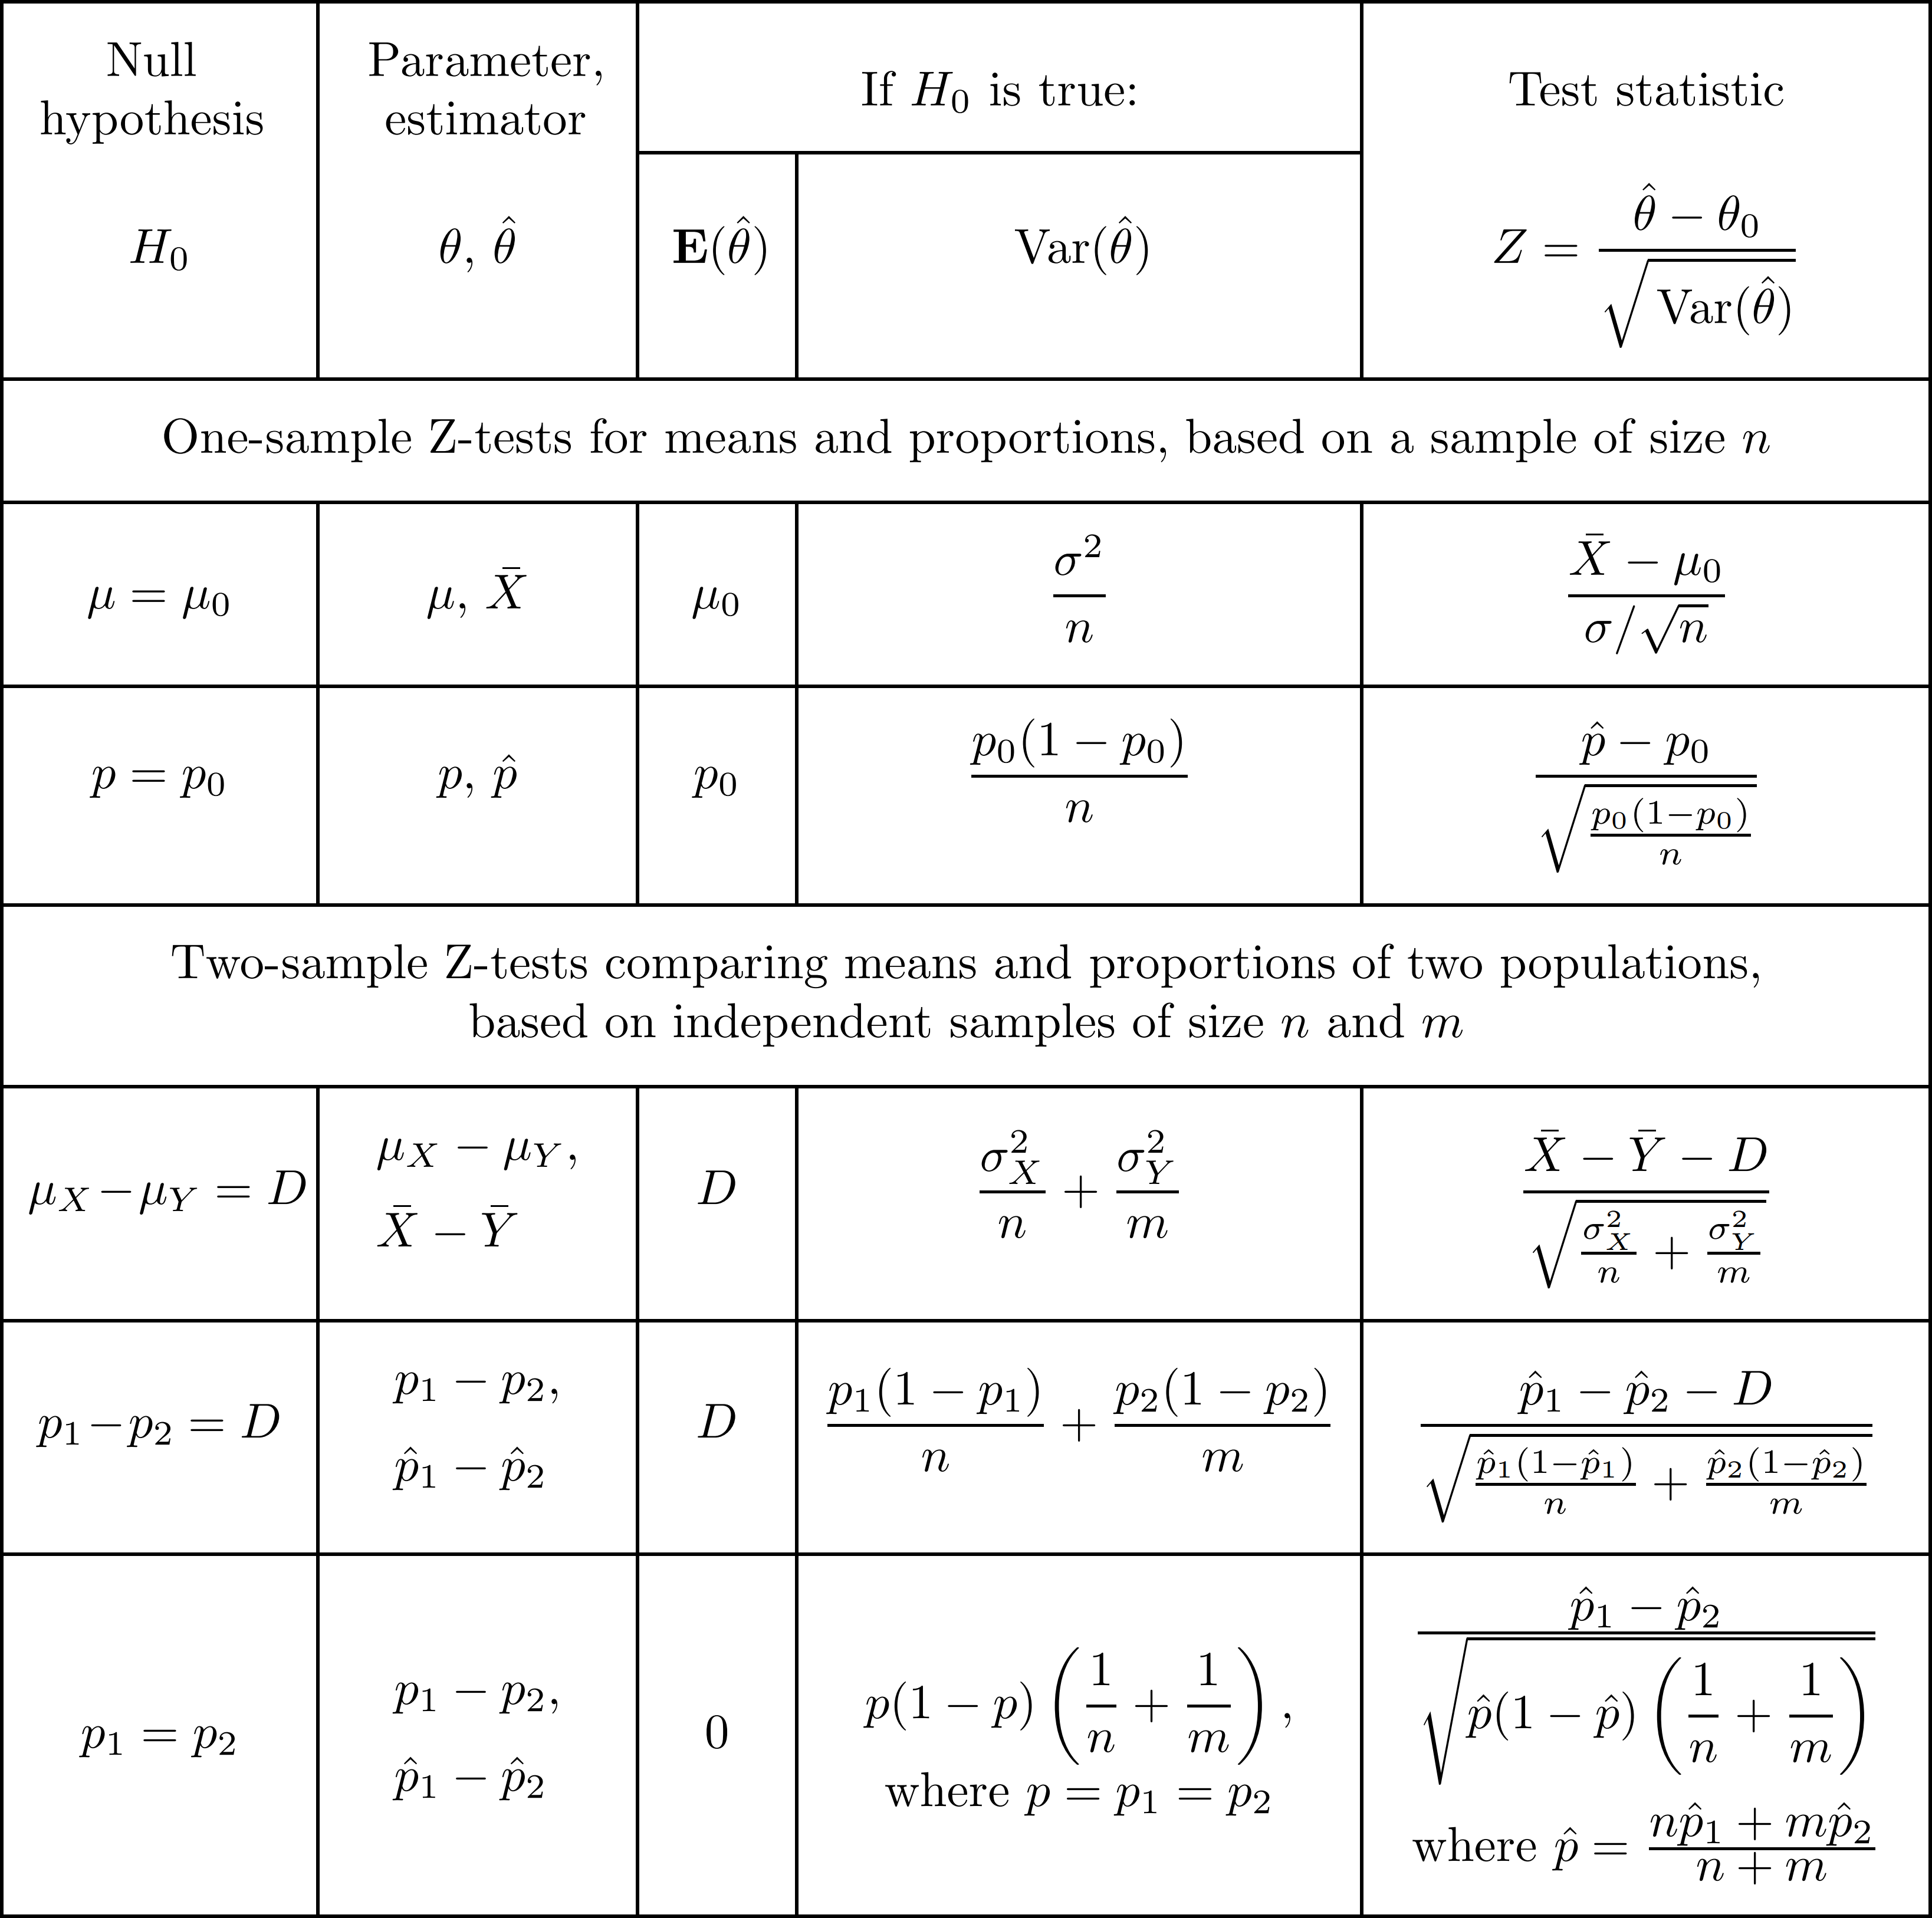
\includegraphics[width=\linewidth]{img/table-9.1.png}
  \caption*{\textbf{Table 1:} \textit{Summary of Z-tests}}
\end{figure}

\newpage

\begin{multicols}{2}
\setlength{\columnsep}{1.5cm}
\setlength{\columnseprule}{0.2pt}

\begin{example}{ (Z-test about a population mean)}
  The number of concurrent users for some internet service provider has always averaged 5000 with a standard deviation of 800. After an equipment upgrade, the average number of users at 100 randomly selected moments of time is 5200. Does it indicate, at a $5\%$ level of significance, that the mean number of concurrent users has increased? Assume that the standard deviation of the number of concurrent users has not changed.

  \textbf{Solution:}
  We test the null hypothesis $H_0\ :\ \mu = 5000$ against a one-sided right-tail alternative $H_A\ :\ \mu > 5000$, because we are only interested to know if the mean number of users $\mu$ has increased.

  \textbf{Step 1:} Test statistic. We are given $\sigma = 800$, $n = 100$, $\alpha = 0.05$, $\mu_0 = 5000$, and from sample, $\bar{X} = 5200$. The test statistic is
  \begin{equation*}
    Z = \frac{\bar{X} - \mu_0}{\sigma / \sqrt{n}} = \frac{5200 - 5000}{800 / \sqrt{100}} = 2.5
  \end{equation*}

  \textbf{Step 2:} Acceptance and rejection regions. The critical value is
  \begin{equation*}
    z_{\alpha} = z_{0.05} = 1.645
  \end{equation*}
  (don't divide $\alpha$ by 2 because it is a one-sided test). With the right-tail alternative, we
  \begin{equation*}
    \begin{cases}
      \textnormal{reject } H_0 &\textnormal{if } Z \geq 1.645\\
      \textnormal{accept } H_0 &\textnormal{if } Z < 1.645\\
    \end{cases}
  \end{equation*}

  \textbf{Step 3:} Result. Our test statistic $Z = 2.5$ belongs to the rejection region; therefore, we reject the null hypothesis. The data (5200 users, on the average, at 100 times) provided sufficient evidence in favor of the alternative hypothesis that the mean number of users has increased.
\end{example}

\begin{example}{ (Two-sample Z-test of proportions)}
  A quality inspector finds 10 defective parts in a sample of 500 parts received from manufacturer A. Out of 400 parts from manufacturer B, she finds 12 defective ones. A computer-making company uses these parts in their computers and claims that the quality of parts produced by A and B is the same. At the $5\%$ level of significance, do we have enough evidence to disprove this claim?

  \textbf{Solution:}
  We test $H_0\ :\ p_A = p_B$, or $H_0\ :\ p_A - p_B = 0$, against $H_A\ :\ p_A \neq p_B$. This is a two-sided test because no direction of the alternative has been indicated. We only need to verify whether or not the proportions of defective parts are equal for manufacturers A and B.

  \textbf{Step 1:} Test statistic. We are given $\\hat{p}_A = 10/500 = 0.02$ from sample size $n = 500$; $\hat{p}_B = 12/400 = 0.03$ from sample size $m = 400$. The tested value is $D = 0$.

  As we know, for these Bernoulli data, the variance depends on the unknown parameters $p_A$ and $p_B$ which are estimated by the sample proportions $\hat{p}_A$ and $\hat{p}_B$.

  The test statistic then equals
  \begin{align*}
    Z &= \dfrac{\hat{p}_A - \hat{p}_B - D}{\sqrt{\dfrac{\hat{p}_A (1 - \hat{p}_A)}{n} + \dfrac{\hat{p}_B (1 - \hat{p}_B)}{m}}} \\
    &= \dfrac{0.02 - 0.03}{\sqrt{\dfrac{(0.02)(0.98)}{500} + \dfrac{(0.03)(0.97)}{400}}} = -0.945
  \end{align*}

  \textbf{Step 2:} Acceptance and rejection regions. This is a two-sided test; thus we divide $\alpha$ by 2, find $z_{0.05/2} = z_{0.025} = 1.96$, and
  \begin{equation*}
    \begin{cases}
      \textnormal{reject } H_0 &\textnormal{if } |Z| \geq 1.96\\
      \textnormal{accept } H_0 &\textnormal{if } |Z| < 1.96\\
    \end{cases}
  \end{equation*}

  \textbf{Step 3:} Result. The evidence against $H_0$ is insufficient because $|Z| < 1.96$. Although sample proportions of defective parts are unequal, the difference between them appears too small to claim that population proportions are different.
\end{example}
